%\documentclass[12pt,a4paper]{article} % POUR TEST
%\usepackage[french]{babel} % POUR TEST
%\usepackage[latin1]{inputenc} % POUR TEST
%\usepackage[T1]{fontenc} % POUR TEST
%\usepackage[UTF8]{inputenc} % POUR TEST
%\usepackage{vmargin} % POUR TEST
%\usepackage{pdfpages} % POUR TEST
%\setmarginsrb{2.5cm}{1.5cm}{2.5cm}{2cm}{0cm}{0cm}{0cm}{0cm} % POUR TEST

%\begin{document} % POUR TEST
\pagestyle{empty}
{\sffamily
\noindent{Universit\'{e} de Lille \hfill Facult\'{e} de Pharmacie de Lille \\ Ann\'{e}e Universitaire 2022/2023}

\vspace{20mm}
\begin{center}
\textbf{THESE \\
POUR LE DIPLOME D'ETAT \\
DE DOCTEUR EN PHARMACIE}
\end{center}
\vspace{10mm}
\noindent{\textbf{\hspace*{13mm}Soutenue publiquement le 12 septembre 2023 \\
\hspace*{11mm}Par M. RIHANI Emir Ka\"{i}s}}
\vspace{22mm}
\begin{center}
\rule{65mm}{0.8pt} \\
\vspace{4mm}
\textbf{APPLICATION DE MODELES D'APPRENTISSAGE MACHINE \\~\\ A LA CLASSIFICATION DES MACROMYCETES} \\
\vspace{2mm}
\rule{65mm}{0.8pt}
\end{center}
\vspace{32mm}
\noindent{\textbf{\underline{\smash{Membres du jury}} :} \\
~\\
\textbf{Pr\'{e}sident :} \\ 
Pr LEMDANI Mohammed, PU en Biomath\'{e}matiques, Facult\'{e} de Pharmacie de Lille \\
~\\
\textbf{Directeur, conseiller de th\`{e}se :} \\
Dr HAMONIER Julien, MCU en Biomath\'{e}matiques, Facult\'{e} de Pharmacie de Lille \\
~\\
\textbf{Assesseur :} \\
Dr WELTI St\'{e}phane, MCU en Sciences V\'{e}g\'{e}tales et Fongiques, Facult\'{e} de Pharmacie de Lille \\
~\\
\textbf{Membre extérieur :} \\
Dr MOUSSET Caroline, Pharmacien-Ing\'{e}nieur, Responsable AQ Clients, Delpharm Lille
}
\newpage
~ % page blanche verso de couverture

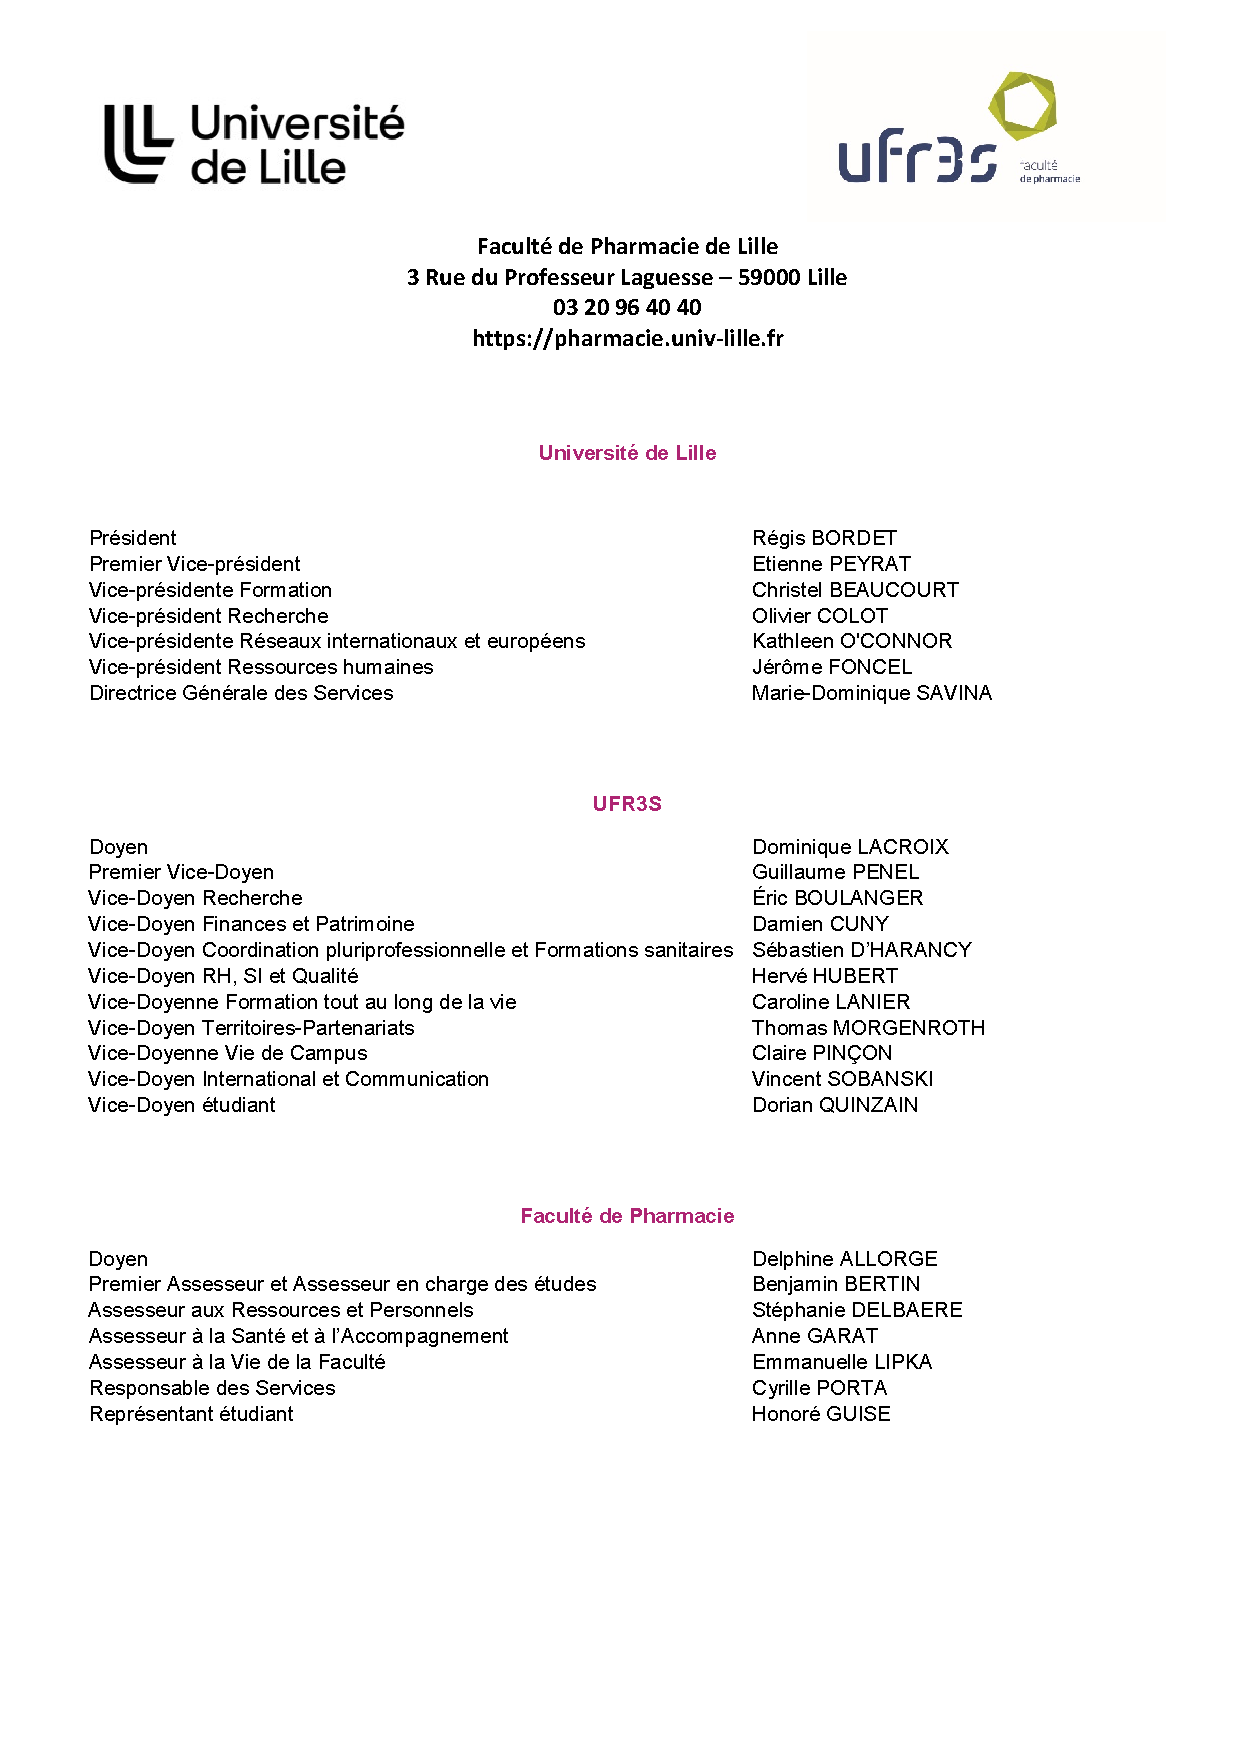
\includepdf[pages={-}]{fac-enseignants2022.pdf} % liste des profs
\newpage
~ % page blanche verso liste des profs

\newpage

\includepdf[pages={-}]{fac-disclaimer.pdf} % disclaimer opinions
\newpage
~ % page blanche verso disclaimer

\newpage
{\rmfamily
~ \\ ~
J'adresse mes sincères remerciements :
\vspace{2cm}
{\itshape 
%Au Professeur Mohammed \textsc{Lemdani}, qui me fait l'honneur de présider mon jury de thèse.
%\paragraph*{}
%Au Dr Julien \textsc{Hamonier}, qui a accepté d'encadrer cette thèse. Merci Julien, pour ton soutien et tes précieux conseils au cours de la réalisation de cet ouvrage.
%\paragraph*{}
%Aux Dr Stéphane \textsc{Welti} et Caroline \textsc{Mousset}, qui me font le plaisir d'intégrer ce jury de thèse. Merci, cher Stéphane, chère Caroline, pour m'avoir enseigné et accompagné durant cette thèse et bien %d'autres projets.
%\paragraph*{}
%Au Pr Régis \textsc{Courtecuisse} pour ses encouragements, sa bienveillance envers ses étudiants et -- bien entendu -- pour ses ouvrages de référence sans lesquels cette thèse n'aurait pu voir le jour.

A la dream-team de tous ceux que je vais remercier.
}
}
\newpage
~ %page blanche verso de remerciements

\newpage %début document (sommaire)
%\end{document} % POUR TEST
